% Search for all the places that say "PUT SOMETHING HERE".

\documentclass[11pt]{article}
\usepackage{amsmath,textcomp,amssymb,graphicx,enumerate,hyperref,enumitem,mathtools,tikz-qtree,listings,chemformula,bm,graphicx,grffile,gensymb,physics,amssymb,datetime,siunitx,multicol}
\graphicspath{{/Users/jonathansun5/Documents/Fall 2017/MCB 166/Homeworks/HW 4/Screen Shot 2017-10-29 at 5.24.09 PM.png} {/Users/jonathansun5/Documents/Fall 2017/MCB 166/Homeworks/HW 4/Screen Shot 2017-10-29 at 5.46.54 PM.png} {/Users/jonathansun5/Documents/Fall 2017/MCB 166/Homeworks/HW 4/Screen Shot 2017-10-30 at 3.38.00 AM.png} {/Users/jonathansun5/Documents/Fall 2017/MCB 166/Homeworks/HW 4/Screen Shot 2017-10-30 at 9.18.49 PM.png} {/Users/jonathansun5/Documents/Fall 2017/MCB 166/Homeworks/HW 4/Screen Shot 2017-10-30 at 9.19.05 PM.png} {/Users/jonathansun5/Documents/Fall 2017/MCB 166/Homeworks/HW 4/Screen Shot 2017-10-30 at 9.19.31 PM.png} {/Users/jonathansun5/Documents/Fall 2017/MCB 166/Homeworks/HW 4/Screen Shot 2017-10-30 at 9.19.43 PM.png} {/Users/jonathansun5/Documents/Fall 2017/MCB 166/Homeworks/HW 4/Screen Shot 2017-10-30 at 9.20.00 PM.png} {/Users/jonathansun5/Documents/Fall 2017/MCB 166/Homeworks/HW 4/Screen Shot 2017-10-31 at 4.37.04 AM.png} {/Users/jonathansun5/Documents/Fall 2017/MCB 166/Homeworks/HW 4/Screen Shot 2017-10-31 at 4.37.21 AM.png} {/Users/jonathansun5/Documents/Fall 2017/MCB 166/Homeworks/HW 4/Screen Shot 2017-10-31 at 7.23.24 AM.png} {/Users/jonathansun5/Documents/Fall 2017/MCB 166/Homeworks/HW 4/Screen Shot 2017-10-31 at 7.23.39 AM.png} {/Users/jonathansun5/Documents/Fall 2017/MCB 166/Homeworks/HW 4/Screen Shot 2017-10-31 at 9.45.43 AM.png} {/Users/jonathansun5/Documents/Fall 2017/MCB 166/Homeworks/HW 4/Screen Shot 2017-10-31 at 10.44.52 AM.png}}

\makeatletter
\newcommand{\leqnos}{\tagsleft@true\let\veqno\@@leqno}
\newcommand{\reqnos}{\tagsleft@false\let\veqno\@@eqno}
\reqnos
\makeatother

\def\Name{Jonathan Sun}  % Your name
\def\SID{25020651}  % Your student ID number
\def\Homework{4} % Number of Homework
\def\Session{Fall 2017}


\title{MCB166 --- \Session --- Problem Set \Homework}
\author{\Name, SID \SID}
\markboth{MCB166 --- \Session --- Problem Set \Homework --- \Name}{MCB166 --- \Session --- Problem Set \Homework --- \Name}
\pagestyle{myheadings}
\newdate{date}{31}{10}{2017}
\date{\displaydate{date}}

\def\endproofmark{$\Box$}
\newenvironment{proof}{\par{\bf Proof:}}{\endproofmark\smallskip}

\usepackage[margin=1in]{geometry}



\begin{document}
\maketitle

\newpage
\begin{enumerate}[label=\arabic*.]
\item
\underline{Hodgkin-Huxley axon. Conditions for a potassium negative conductance.}
\\
The HH equations for a space-clamped squid giant axon are given below. Tetrodotoxin (TTX), the puffer-fish poison is known to block axonal \ch{Na} channels. When TTX is introduced into the bathing medium, the axon $I_{\ch{Na}}$ will be blocked and $I_{\ch{K}}$ and $I_{\ch{L}}$ will remain unchanged. Ordinarily, the nerve would be incapable of generating action potentials. We wish to consider an axon bathed in TTX for two different conditions of external \ch{K} concentration --- normal $[\ch{K}]_o$, for which $V_{\ch{K}} = -75 \text{mV}$, and high $[\ch{K}]_o$, for which $V_{\ch{K}} = 0$.
\\
The conductance, $\overline{g}_{\ch{K}}$ might also vary with changed external \ch{K}, but for the sake of simplicity, we will assume $\overline{g}_{\ch{K}}$ does not change.
\begin{center}
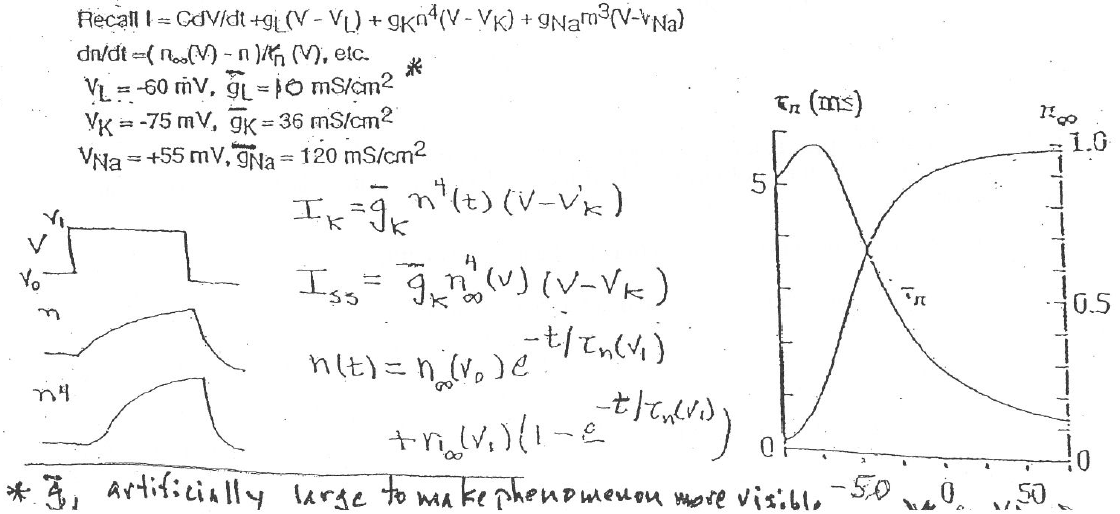
\includegraphics[width=0.75\textwidth]{/Users/jonathansun5/Documents/Fall 2017/MCB 166/Homeworks/HW 4/Screen Shot 2017-10-31 at 9.45.43 AM.png}
\end{center}
\begin{enumerate}[label=(\alph*)]
\item
In a voltage clamp experiment, the membrane potential is held for a long time at a potential $V = -100 \text{mV}$, and then a depolarizing step of $60 \text{mV}$ to $V = 40 \text{mV}$ is applied for $30 \text{msec}$. By integrating the equation for $n(t)$ for the appropriate boundary conditions, solve for the time course of $\overline{g}_{\ch{K}}$. Show mathematically that the rising phase of the conductance has an inflection point but that the falling phase does not. This delayed onset but undelayed fall is what Hodgkin and Huxley originally required for the time-dependent conductances. You may assume $n_{\infty}(-100) = 0$; $\tau_n(-100) = 5 \text{msec}$ throughout.
\begin{align*}
n_{\infty}(-100 \text{mV}) = 0
\end{align*}
\begin{align*}
\tau_{n}(-100 \text{mV}) = 5 \text{msec}
\end{align*}
\begin{align*}
n_{\infty}(-40 \text{mV}) = 0.75
\end{align*}
\begin{align*}
\tau_{n}(-40 \text{mV}) = 3 \text{msec}
\end{align*}
Upstep:
\\
Since $n(t) = n_{\infty}(V_0) e^{\frac{-t} {\tau_n(V_1)}} + n_{\infty}(V_1) \left(1 - e^{\frac{-t} {\tau_n(V_1)}}\right)$, we get:
\begin{align*}
n(t) = 0 + 0.75 \left(1 - e^{\frac{-t} {3}}\right) = 0.75 \left(1 - e^{\frac{-t} {3}}\right)
\end{align*}
Since $I_{\ch{K}} = \overline{g}_{\ch{K}} n^4(t) (V - V_k)$:
\begin{align*}
I_{\ch{K}} = \overline{g}_{\ch{K}} \left(0.75 \left(1 - e^{\frac{-t} {3}}\right)\right)^4
\end{align*}
Since the depolarizing step is applied for only $30 \text{msec}$ and $\overline{g}_{\ch{K}} = 36 \frac{\text{mS}} {\text{cm}^2}$:
\begin{align*}
I_{\ch{K}} = 36 \left(0.75 \left(1 - e^{\frac{-30} {3}}\right)\right)^4 = 11.389 \frac{\text{mS}} {\text{cm}^2}
\end{align*}
Downstep:
\\
Since $n(t) = n_{\infty}(V_0) e^{\frac{-t} {\tau_n(V_1)}} + n_{\infty}(V_1) \left(1 - e^{\frac{-t} {\tau_n(V_1)}}\right)$, we get:
\begin{align*}
n(t) = 0.75 e^{\frac{-t} {5}} + 0 = 0.75 e^{\frac{-t} {5}}
\end{align*}
Thus:
\begin{align*}
I_{\ch{K}} = \overline{g}_{\ch{K}} \left(0.75 e^{\frac{-t} {5}}\right)^4 = 36 \left(0.75 e^{\frac{-t} {5}}\right)^4
\end{align*}
To solve for the inflection point we first have:
\begin{align*}
g_{\ch{K}} = \overline{g}_{\ch{K}} \left(0.75 \left(1 - e^{\frac{-t} {3}}\right)\right)^4
\end{align*}
Next, we solve for:
\begin{align*}
\frac{d} {dt} \left(0.75 \left(1 - e^{\frac{-t} {3}}\right)\right)^4 &= 4 \left(1 - e^{\frac{-t} {3}}\right) \frac{d} {dt} \left(1 - e^{\frac{-t} {3}}\right) \\
&= 4 \left(1 - e^{\frac{-t} {3}}\right)^3 \left(- e^{\frac{-t} {3}} \times \frac{-1} {3}\right) \\
&= \frac{4} {3} e^{\frac{-t} {3}} \left(1 - e^{\frac{-t} {3}}\right)^3
\end{align*}
\begin{align*}
\frac{d^2} {d^2t} \left(1 - e^{\frac{-t} {3}}\right)^4 &= \frac{4} {3} \left(-\frac{1} {3} e^{\frac{-t} {3}}\right) \left(1 - e^{\frac{-t} {3}}\right)^3 + \frac{4} {3} e^{\frac{-t} {3}} \times 3 \left(1 - e^{\frac{-t} {3}}\right)^2 \times \left(\frac{1} {3} e^{\frac{-t} {3}}\right) \\
&= -\frac{4} {9} e^{\frac{-t} {3}} \left(1 - e^{\frac{-t} {3}}\right)^3 + \frac{4} {3} e^{\frac{-2t} {3}} \left(1 - e^{\frac{-t} {3}}\right)^2 = 0
\end{align*}
\begin{align*}
\frac{1} {3} - \frac{1} {3} e^{\frac{-t} {3}} = e^{\frac{-t} {3}}
\end{align*}
\begin{align*}
\frac{1} {3} = \frac{4} {3} e^{\frac{-t} {3}}
\end{align*}
\begin{align*}
\frac{1} {4} = e^{\frac{-t} {3}}
\end{align*}
\begin{align*}
t = -3 \log{\frac{1} {4}}
\end{align*}
So, we get:
\begin{align*}
g_{\ch{K}}\left(t = -3 \log{\frac{1} {4}}\right) = 36 \left(0.75 \left(1 - e^{\frac{3 \log{\frac{1} {4}}} {3}}\right)\right)^4 = 3.6 \frac{\text{mS}} {\text{cm}^2}
\end{align*}
So, the inflection point is $I\left(-3 \log{\frac{1} {4}} \text{, } 3.6\right)$.



\item
Using the plot of part (a) sketch the current $I_{\ch{K}}$ for this voltage pulse for both conditions of $[\ch{K}]_o$ (ie. $V_k = -75$ and $V_k = 0$). Compare the currents during rising and falling phases of conductance for the two conditions. Is $I_{\ch{K}}$ outward for both conditions? Explain. The current transient at the termination of the pulse is called the tail current.
\vspace*{1\baselineskip}
\\
At the step up, the driving force is $-40 \text{mV} - E_{\ch{K}} = -40 \text{mV} + 75 \text{mV} = 35 \text{mV}$. At the step down, the driving force is $-100 \text{mV} + 75 \text{mV} = -25 \text{mV}$. So at the step up, $I_{\ch{K}} = 35 \overline{g}_{\ch{K}}(0.75)^4 = 35 \times 36 \times (0.75)^4 = 398.67 \text{mA}$.
\begin{center}
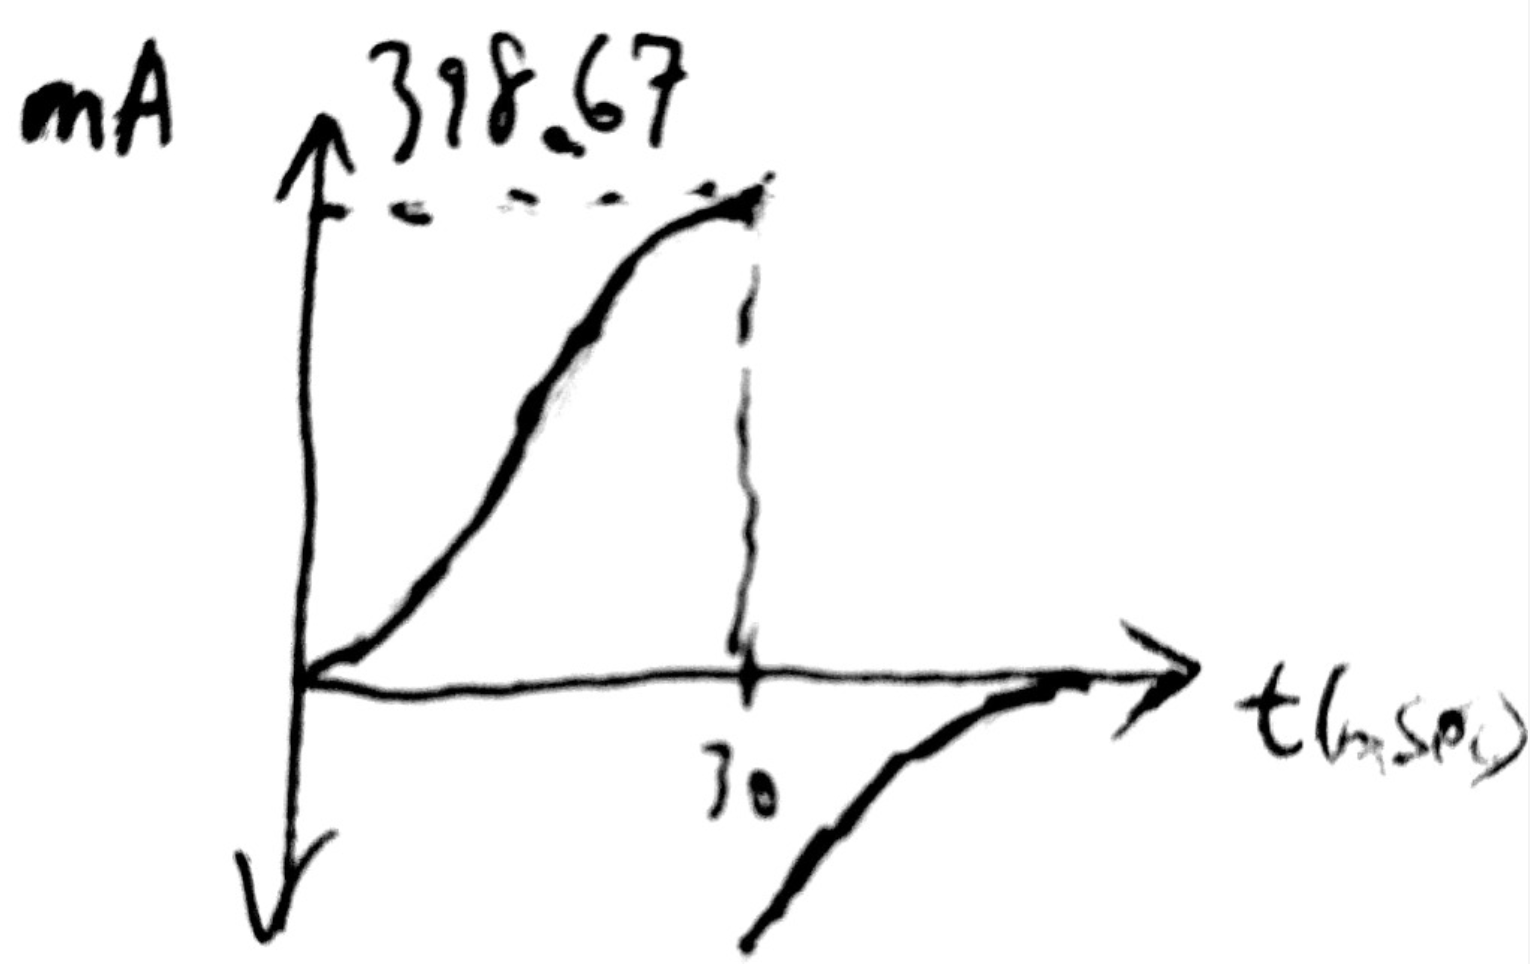
\includegraphics[width=0.75\textwidth]{/Users/jonathansun5/Documents/Fall 2017/MCB 166/Homeworks/HW 4/Screen Shot 2017-10-31 at 10.44.52 AM.png}
\end{center}







\item
For the two conditions of external \ch{K} concentration, plot the steady-state current-voltage relations. Which condition gives a negative conductance? Explain how a negative conductance can come about in the absence of \ch{Na} ions. (Assume that $V_L$ and $\overline{g}_{L}$ are not altered by the ionic changes).
















\item
Can the system in high $[\ch{K}]_o$ give an action potential in response to a short shock of current? If not, can you think of a way of producing a potassium action potential with this system? What would an imposed steady current do?

















\end{enumerate}



\newpage
\item
An alga \textit{Chara globularis} is known to generate positive-going action potentials. The major ions in both its cytoplasma and the pond water it lives in are \ch{Na+}, \ch{K+}, and \ch{CI-}, and their concentrations are as follows:
\begin{center}
	\begin{tabular}{c c c} 
	 & Cytoplasma (mM) & Pond Water (mM) \\ [1ex] 
	\hline
	\ch{Na+} & 57 & 0.031 \\ 
	\ch{K+} & 65 & 0.046 \\
	\ch{Cl-} & 112 & 0.040 \\
	\end{tabular}
\end{center}
The resting potential of the cell is $-182 \text{mV}$, and the peak amplitude of the action potential is $+198 \text{mV}$.
\begin{enumerate}[label=(\alph*)]
\item
What is (are) the primary permeable ion(s) for this cell at rest?
\vspace*{1\baselineskip}
\\
Since $E_{\ch{Na}} = 58 \log{\frac{0.031} {57}} = -189.342 \text{mV}$, $E_{\ch{K}} = 58 \log{\frac{0.046} {65}} = -182.709 \text{mV}$, and $E_{\ch{Cl}} = -58 \log{\frac{0.040} {112}} = +199.935 \text{mV}$,and the resting potential of the cell is $-182 \text{mV}$, the cell is primarily permeable to \ch{K+}. This is because $E_{\ch{K}}$ is closest to the resting potential. The cell is also permeable to \ch{Na+} but to a lesser extent and barely permeable  to \ch{Cl-}.
\\



\item
What is (are) the primary permeable ion(s) for this cell during the peak of an action potential?
\vspace*{1\baselineskip}
\\
Since the peak amplitude of the action potential is $+198 \text{mV}$ and $E_{\ch{Cl}} = +199.935 \text{mV}$, the primary permeable ion for this cell is \ch{Cl-}.
\\



\item
In a pump that pumps both $\ch{Na+}$ and $\ch{Cl-}$ into the cell at a ratio of $1 : 1$, what is the contribution of this pump to the resting potential of the cell?
\vspace*{1\baselineskip}
\\
Since the pump pumps both $\ch{Na+}$ and $\ch{Cl-}$ into the cell at a ratio of $1 : 1$ and the charges of both are opposite to each other but the concentration ratio stays the same, the pump is a neutral pump so there is no contribution to the resting potential of the cell.
\\



\item
The voltage-clamp analysis of this cell reveals the following results:
\begin{center}
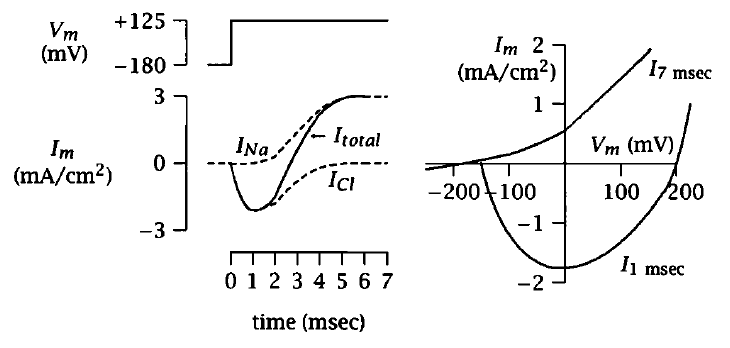
\includegraphics[width=0.75\textwidth]{/Users/jonathansun5/Documents/Fall 2017/MCB 166/Homeworks/HW 4/Screen Shot 2017-10-29 at 5.24.09 PM.png}
\end{center}
What are the values of $g_{\ch{Cl}}$ and $g_{\ch{Na}}$ at $V_m = -50 \text{mV}$ and at $Vm = +150 \text{mV}$?
\vspace*{1\baselineskip}
\\
At $t = 1 \text{msec}$ and $V_m = -50 \text{mV}$:
\begin{align*}
g_{\ch{Cl}} = \frac{-1.7} {-50 - (+199.935)} = 6.8 \text{nS}
\end{align*}
\begin{align*}
g_{\ch{Na}} = \frac{0} {-50 - (-189.342)} = 0 \text{nS}
\end{align*}
At $t = 1 \text{msec}$ and $V_m = +150 \text{mV}$:
\begin{align*}
g_{\ch{Cl}} = \frac{-0.8} {+150 - (+199.935)} = 16.02 \text{nS}
\end{align*}
\begin{align*}
g_{\ch{Na}} = \frac{0} {+150 - (-189.342)} = 0 \text{nS}
\end{align*}
At $t = 7 \text{msec}$ and $V_m = -50 \text{mV}$:
\begin{align*}
g_{\ch{Cl}} = \frac{0} {-50 - (+199.935)} = 0 \text{nS}
\end{align*}
\begin{align*}
g_{\ch{Na}} = \frac{0.3} {-50 - (-189.342)} = 2.15 \text{nS}
\end{align*}
At $t = 7 \text{msec}$ and $V_m = +150 \text{mV}$:
\begin{align*}
g_{\ch{Cl}} = \frac{0} {+150 - (+199.935)} = 0 \text{nS}
\end{align*}
\begin{align*}
g_{\ch{Na}} = \frac{1.9} {+150 - (-189.342)} = 5.599 \text{nS}
\end{align*}
\end{enumerate}



\newpage
\item
Which of the Hodgkin-Huxley variables, $m$, $h$, or $n$ is primarily responsible for each of the following phenomena: Explain your choice in one short sentence.
\begin{enumerate}[label=(\alph*)]
\item
Sharp threshold for excitation (for short-duration stimuli).
\vspace*{1\baselineskip}
\\
The relevant variables are $n$ and $m$ since they are activated by depolarization. Since there is a sharp threshold for excitation, $m$ is more responsible since it is associated with \ch{Na+} channel activation which happens faster than \ch{K+} channel activation which is associated with $n$. Meanwhile, $h$ is less relavent because \ch{K+} channels open slowly.
\\



\item
Rapid repolarization at the end of an action potential.
\vspace*{1\baselineskip}
\\
The relevant variables are $h$ and $m$ since $h$ is inactivated by depolarization and $m$ is associated with \ch{Na+} channel activation. Since there is a rapid repolarization, $m$-gates shut quickly while $h$-gates also shut. Meanwhile, $n$ is less relavent because it slowly shuts when it reaches the peak of the action potential.
\\



\item
Undershoot after an action potential, ie. voltage is temporarily hyperpolarized beyond rest.
\vspace*{1\baselineskip}
\\
The relevant variable is $h$ because during hyperpolarization, $h$-gates open. $m$-gates are still shut during this time.
\\



\item
Anode-break excitation, ie. membrane has lowered threshold after hyperpolarizing prepulse.
\vspace*{1\baselineskip}
\\
The relevant variable is $n$ because it is associated with \ch{K+} channel activation and since the relatively slow rate at which the K channels shut means that it is going to influence the anode-break excitation.
\\
\end{enumerate}



\newpage
\item
The electric organ of the electric eel can generate a $600$ volt discharge. It is made up of stacks of about $4000$ asymmetric disc-shaped cells called electroplaques. The entire stack is surrounded by an insulating sheath, as shown in Fig. $1$. Each electroplaque has two different faces --- A and B in the figure. At rest, both faces are permeable to \ch{K+} and have relatively high resistance. At the peak of the action potential, face A has many activated \ch{Na+} channels, and thus has a low resistance and is permeable to \ch{Na+}. Face B is transiently activated by postsynaptic (acetylcholine) channels to trigger the action potential in face A. The acetylcholine channel is equally permeable to \ch{Na+} and \ch{K+} and has a reversal potential near zero. During activity this face also shows a low resistance.
\begin{center}
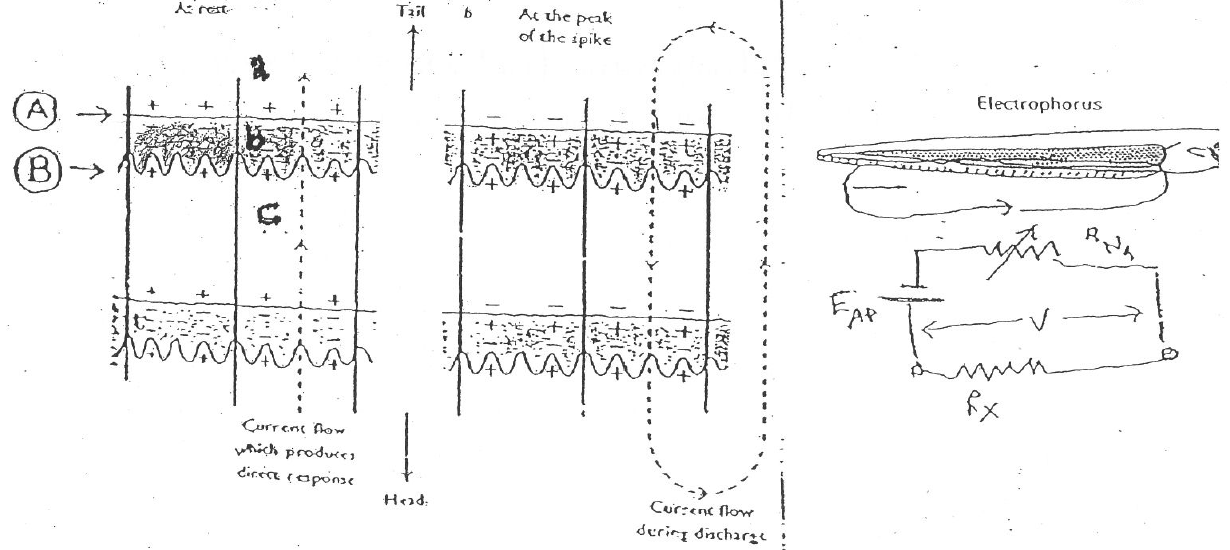
\includegraphics[width=0.75\textwidth]{/Users/jonathansun5/Documents/Fall 2017/MCB 166/Homeworks/HW 4/Screen Shot 2017-10-29 at 5.46.54 PM.png}
\end{center}
\begin{enumerate}[label=(\alph*)]
\item
Draw an equivalent circuit for the cell at rest and at peak activity representing the two membranes in series and using $V_{\ch{Na}} = +50 \text{mV}$ (inside relative to outside) and $V_{\text{rest}} = -90 \text{mV}$ (inside relative to outside). Calculate the resting potential and the action potential peak amplitude measured between microelectrodes placed at points a and b, and then between electrodes placed at a and c. $[\text{amplitude of AP} = V_{\text{AP}} - V_{\text{rest}}]$.
\begin{multicols}{2}
Cell at Rest:
\begin{center}
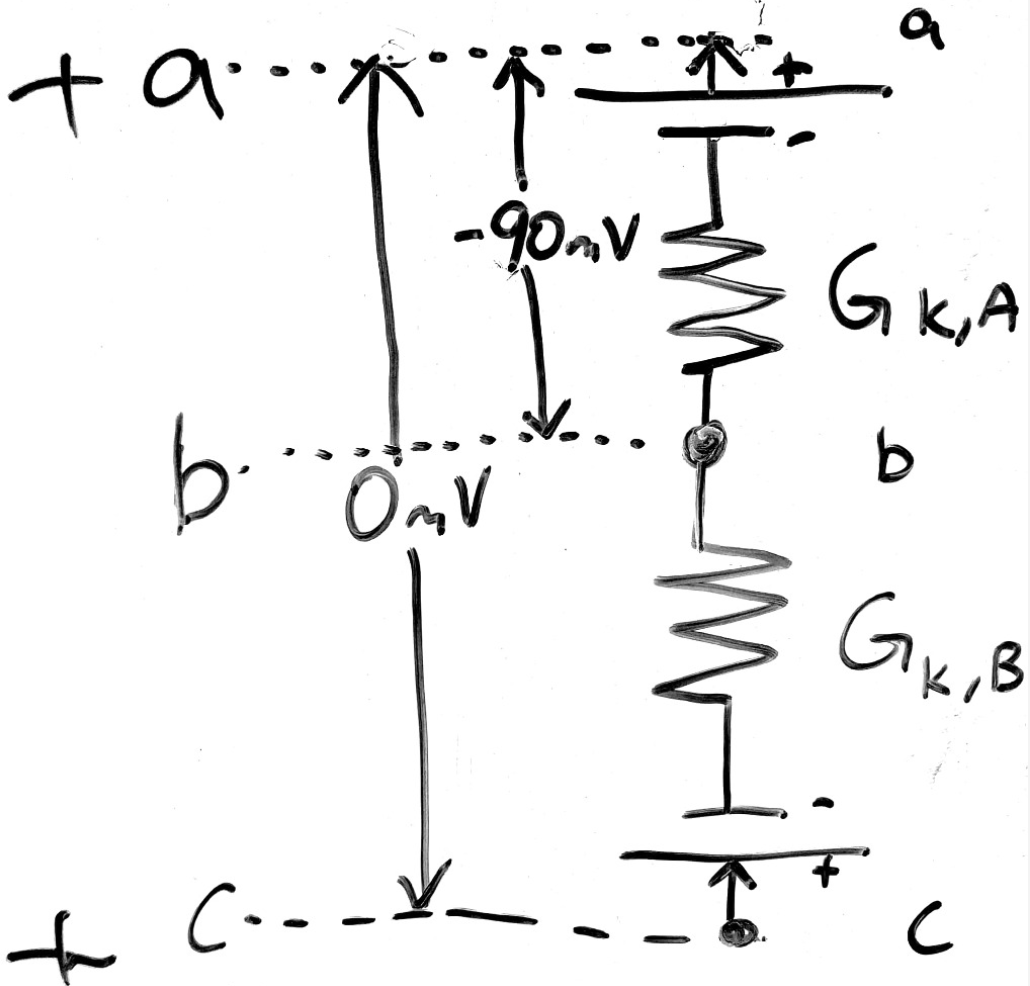
\includegraphics[width=0.5\columnwidth]{/Users/jonathansun5/Documents/Fall 2017/MCB 166/Homeworks/HW 4/Screen Shot 2017-10-31 at 4.37.04 AM.png}
\end{center}
\begin{align*}
V_{a \to b} &= -V_{b \to a} = 90 \text{mV} \\
V_{a \to c} &= V_{a \to b} + V_{b \to c} \\
&= 90 \text{mV} -90 \text{mV} \\
&= 0 \text{mV}
\end{align*}
\medbreak
Cell at Peak Activity:
\begin{center}
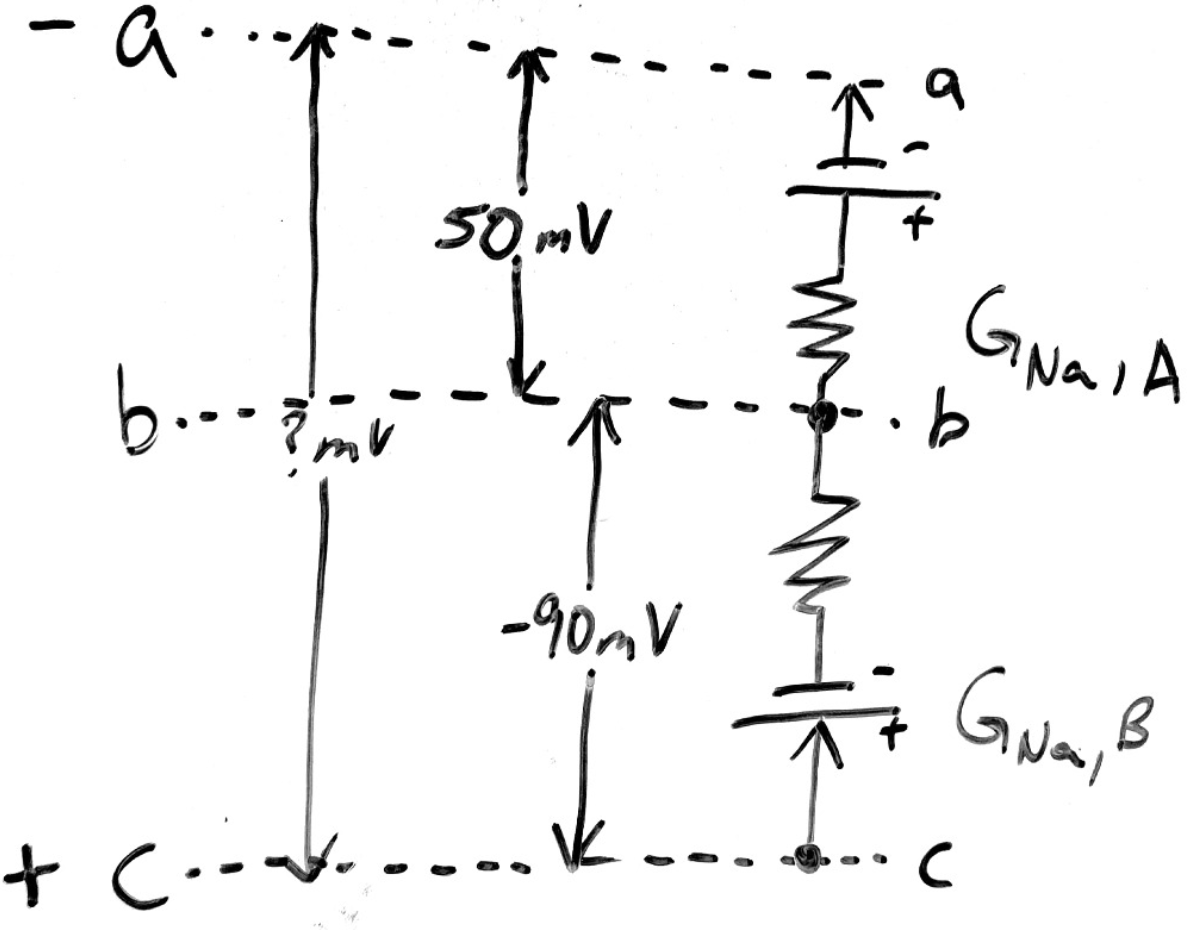
\includegraphics[width=0.5\columnwidth]{/Users/jonathansun5/Documents/Fall 2017/MCB 166/Homeworks/HW 4/Screen Shot 2017-10-31 at 4.37.21 AM.png}
\end{center}
\begin{align*}
V_{b \to a} &= E_{\ch{Na}} = 50 \text{mV} \\
V_{c \to a} &= V_{c \to b} + V_{b \to a} \\
&= -(-90 \text{mV}) + 50 \text{mV} \\
&= 140 \text{mV}
\end{align*}
\end{multicols}
Amplitude of the Action Potential:
\begin{align*}
\text{Amplitude of AP}_{a \to b} = \abs{-50 \text{mV} - 90 \text{mV}} = 140 \text{mV}
\end{align*}
\begin{align*}
\text{Amplitude of AP}_{a \to c} = \abs{-140 \text{mV} - 0 \text{mV}} = 140 \text{mV}
\end{align*}



\item
Using the circuit diagram for a single electric cell, draw and label the equivalent circuit for the entire stack of $4000$ cells. Calculate the voltage drop across the stack at rest and at the action potential peak. Explain why the electric organ can generate such high voltages (sufficient to light up neon lights in aquariums). Why is it unlikely that a single excitable cell can be designed to generate voltages much higher than a few hundred millivolts?
\vspace*{1\baselineskip}
\\
Because the resisters are in series and I would not like to draw the circuit diagrams for each of the cells, I can draw the circuit diagrams after adding up the resistances into one total resistance.
\begin{multicols}{2}
4000 Cells at Rest:
\begin{center}
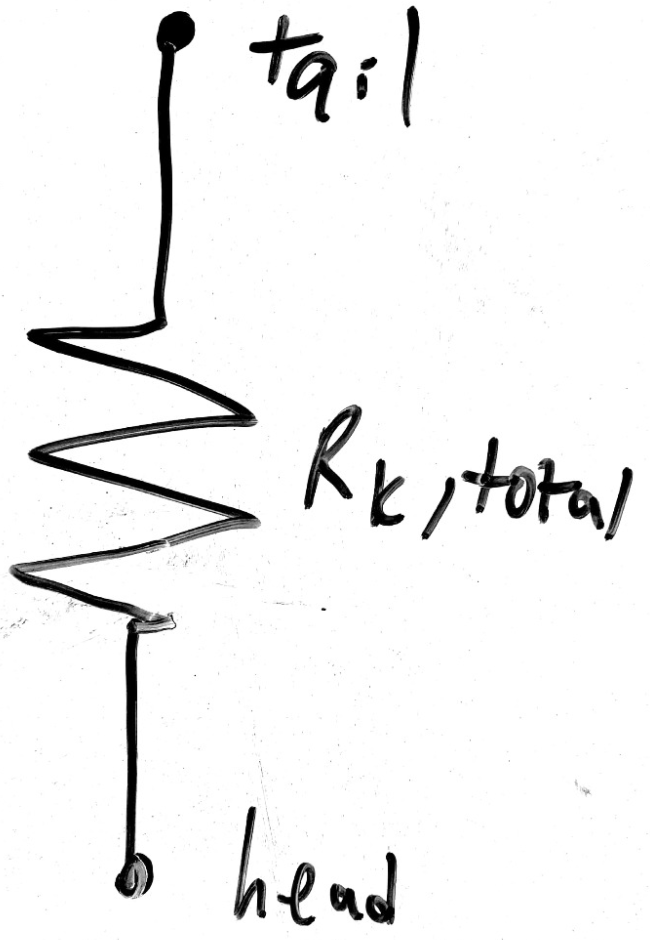
\includegraphics[width=0.5\columnwidth]{/Users/jonathansun5/Documents/Fall 2017/MCB 166/Homeworks/HW 4/Screen Shot 2017-10-31 at 7.23.24 AM.png}
\end{center}
At rest, the total current is $0$ and so the $4000$ cells has $V_{\text{rest, total}} = 0 \text{mV}$.
\medbreak
400 Cells at Peak Activity:
\begin{center}
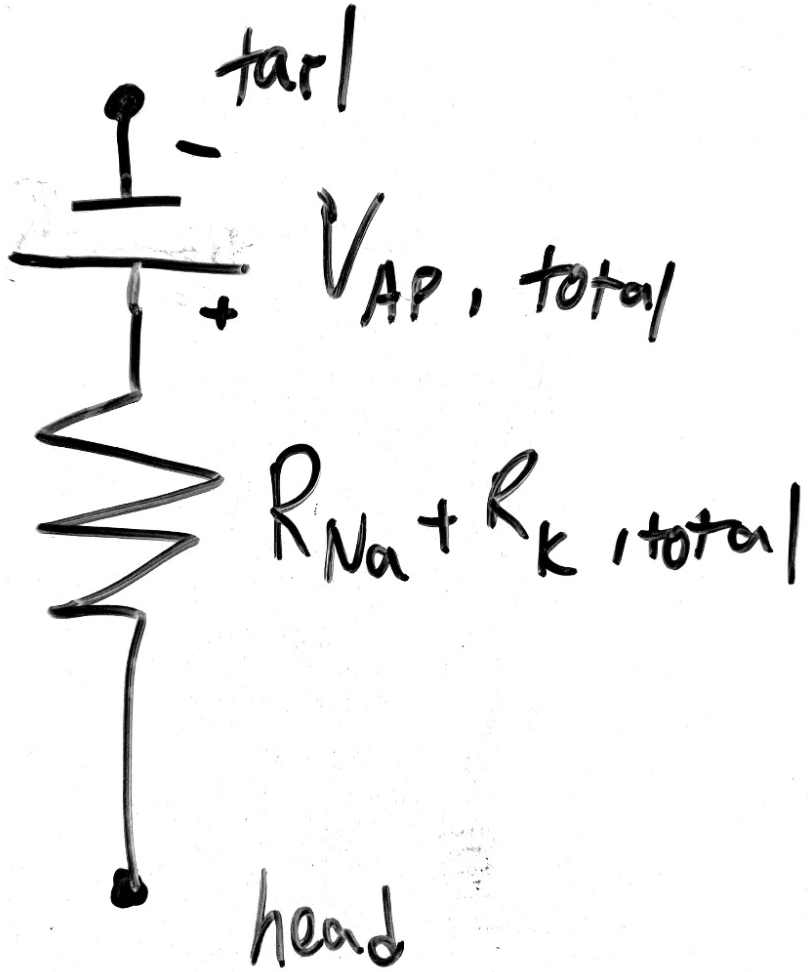
\includegraphics[width=0.5\columnwidth]{/Users/jonathansun5/Documents/Fall 2017/MCB 166/Homeworks/HW 4/Screen Shot 2017-10-31 at 7.23.39 AM.png}
\end{center}
At the peak of the action potential, the $4000$ cells in a series has $V_{\text{AP, total}} = 4000 \times 140 \text{mV} = 560000 \text{mV} = 560 \text{V}$.
\end{multicols}
Since each cell has their own voltage of $140 \text{mV}$, I can add them together since they are in a series. So, an organ with many cells will be able to generate a lot of voltage because the total voltage is the summation of all of the individual voltages in each cell. Therefore, the electric organ can generate high voltages that are sufficien to light up neon lights in aquariums.
\\



\item
Complete the equivalent circuit for an electric organ composed of $4000$ electroplaques at peak discharge by sending current through an external resistance, $R_x$, the resistance of the medium through which the fish swims. Write an expression for the voltage the electric fish can utilize to stun its prey. There are both marine and fresh-water electric fish. Explain why the fresh-water types are more effective at stunning their prey. In fact, marine electric fish have only the excitable synaptic face with no electrically excitable face.
\begin{align*}
\frac{V_{\text{fish}}} {560 \text{V}} = \frac{I R_x} {I R_{\text{eel}} + I R_x}
\end{align*}
face.
\begin{align*}
\frac{V_{\text{fish}}} {560 \text{V}} = \frac{R_x} {R_{\text{eel}} + R_x}
\end{align*}
\begin{align*}
V_{\text{fish}} = \frac{560 R_x} {R_{\text{eel}} + R_x}
\end{align*}
Since fresh-water has higher resistance than seawater, $R_{\text{fresh-water}} > R_{\text{salt-water}}$.  Since the resistance of the seawater is much smaller than the resistance of the fresh-water, there is a stronger electric shock on the prey if it took place in fresh-water as opposed to the current being diverted in seawater.
\end{enumerate}



\newpage
\item
When a normal, healthy squid axon is voltage-clamped in artificial
sea water, one obtains the following membrane current record in response
to a step change in membrane potential from $V_m = -70 \text{mV}$
to $V_m = 0 \text{mV}$.
\begin{center}
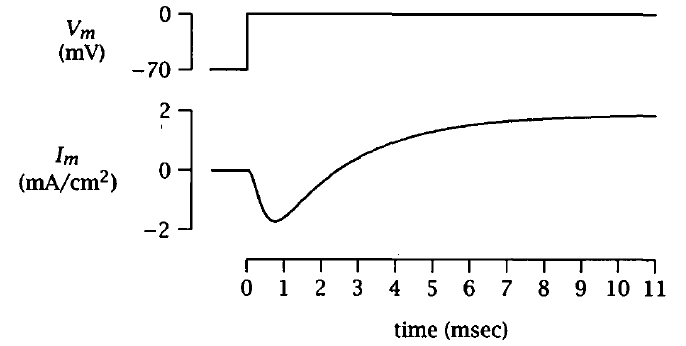
\includegraphics[width=0.75\textwidth]{/Users/jonathansun5/Documents/Fall 2017/MCB 166/Homeworks/HW 4/Screen Shot 2017-10-30 at 3.38.00 AM.png}
\end{center}
Draw similar plots of $I_m$ vs. $t$ (when $V_m$ is stepped from $- 70 \text{mV}$ to $0 \text{mV}$) when the recordings are made under each of the following experimental conditions. For each of your plots, explain in one or two sentences how and why your graph differs from that drawn above.
\begin{enumerate}[label=(\alph*)]
\item
TTX is added to the bath surrounding the axon.
\vspace*{1\baselineskip}
\\
Because tetrodotoxin is a \ch{Na+} channel blocker, the current will not go below 0.
\begin{center}
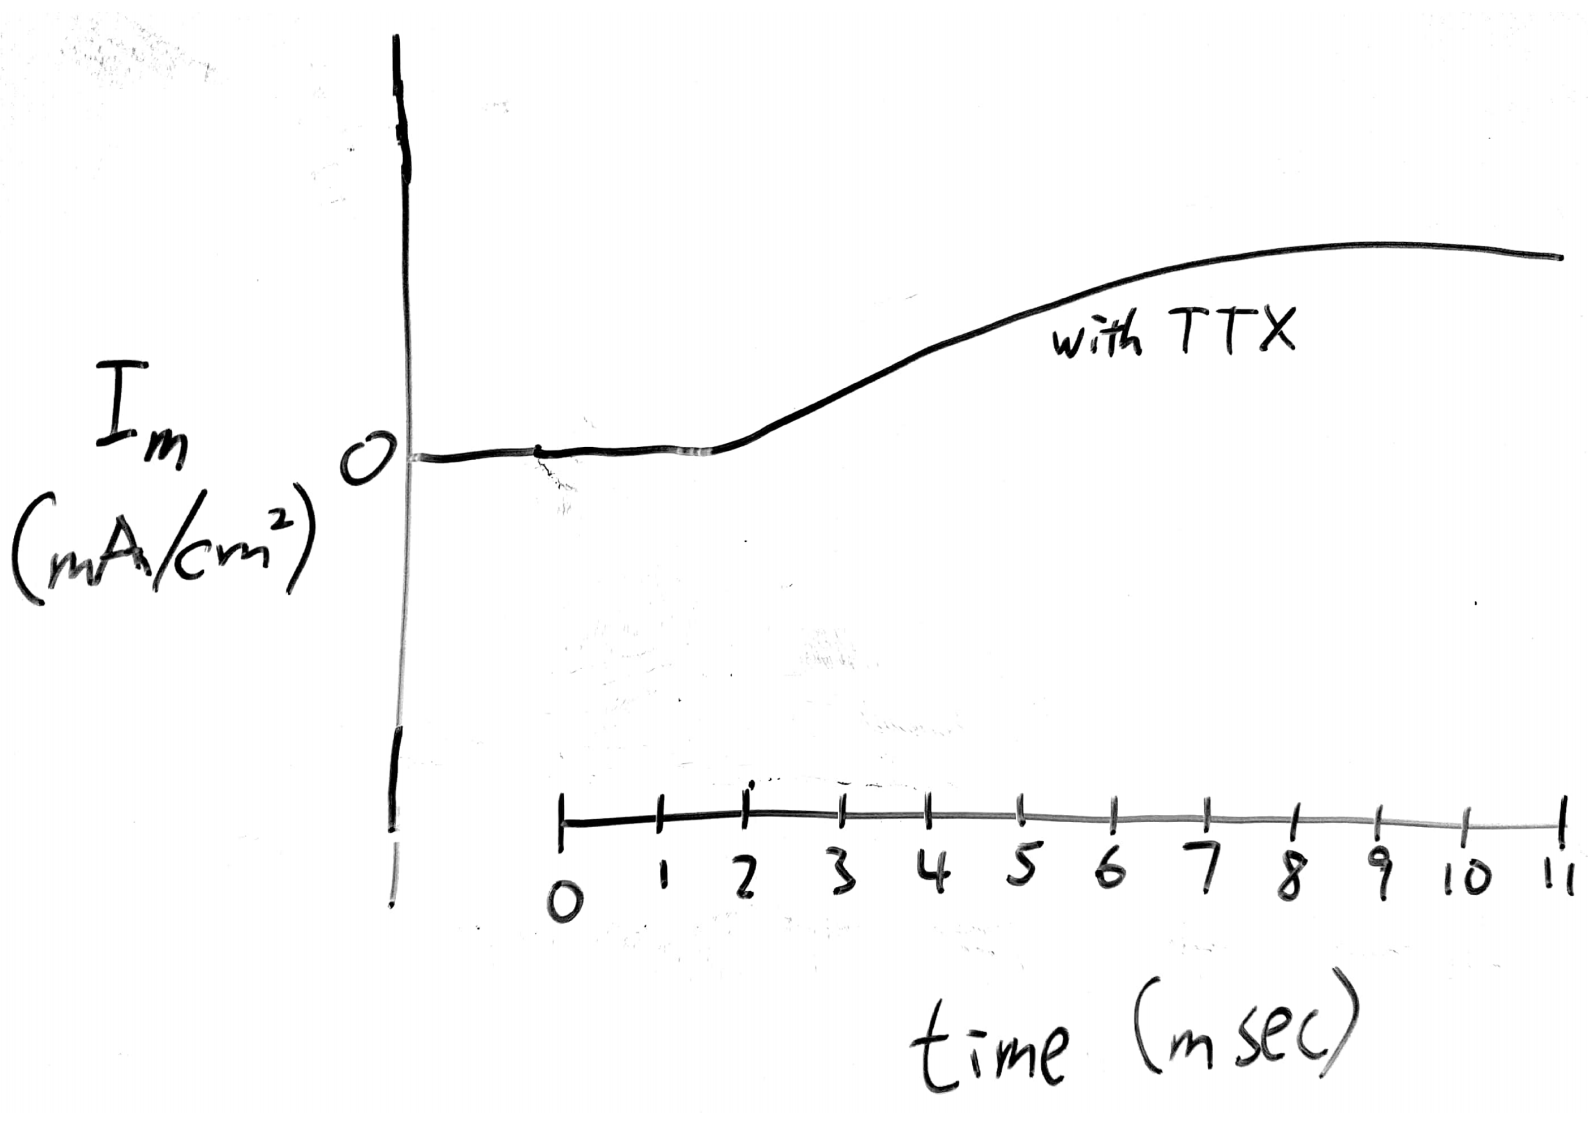
\includegraphics[width=0.5\textwidth]{/Users/jonathansun5/Documents/Fall 2017/MCB 166/Homeworks/HW 4/Screen Shot 2017-10-30 at 9.18.49 PM.png}
\end{center}



\item
TEA is added to the interior of the axon.
\vspace*{1\baselineskip}
\\
Because tetraethylammonium is a \ch{K+} channel blocker, the current will not go above 0.
\begin{center}
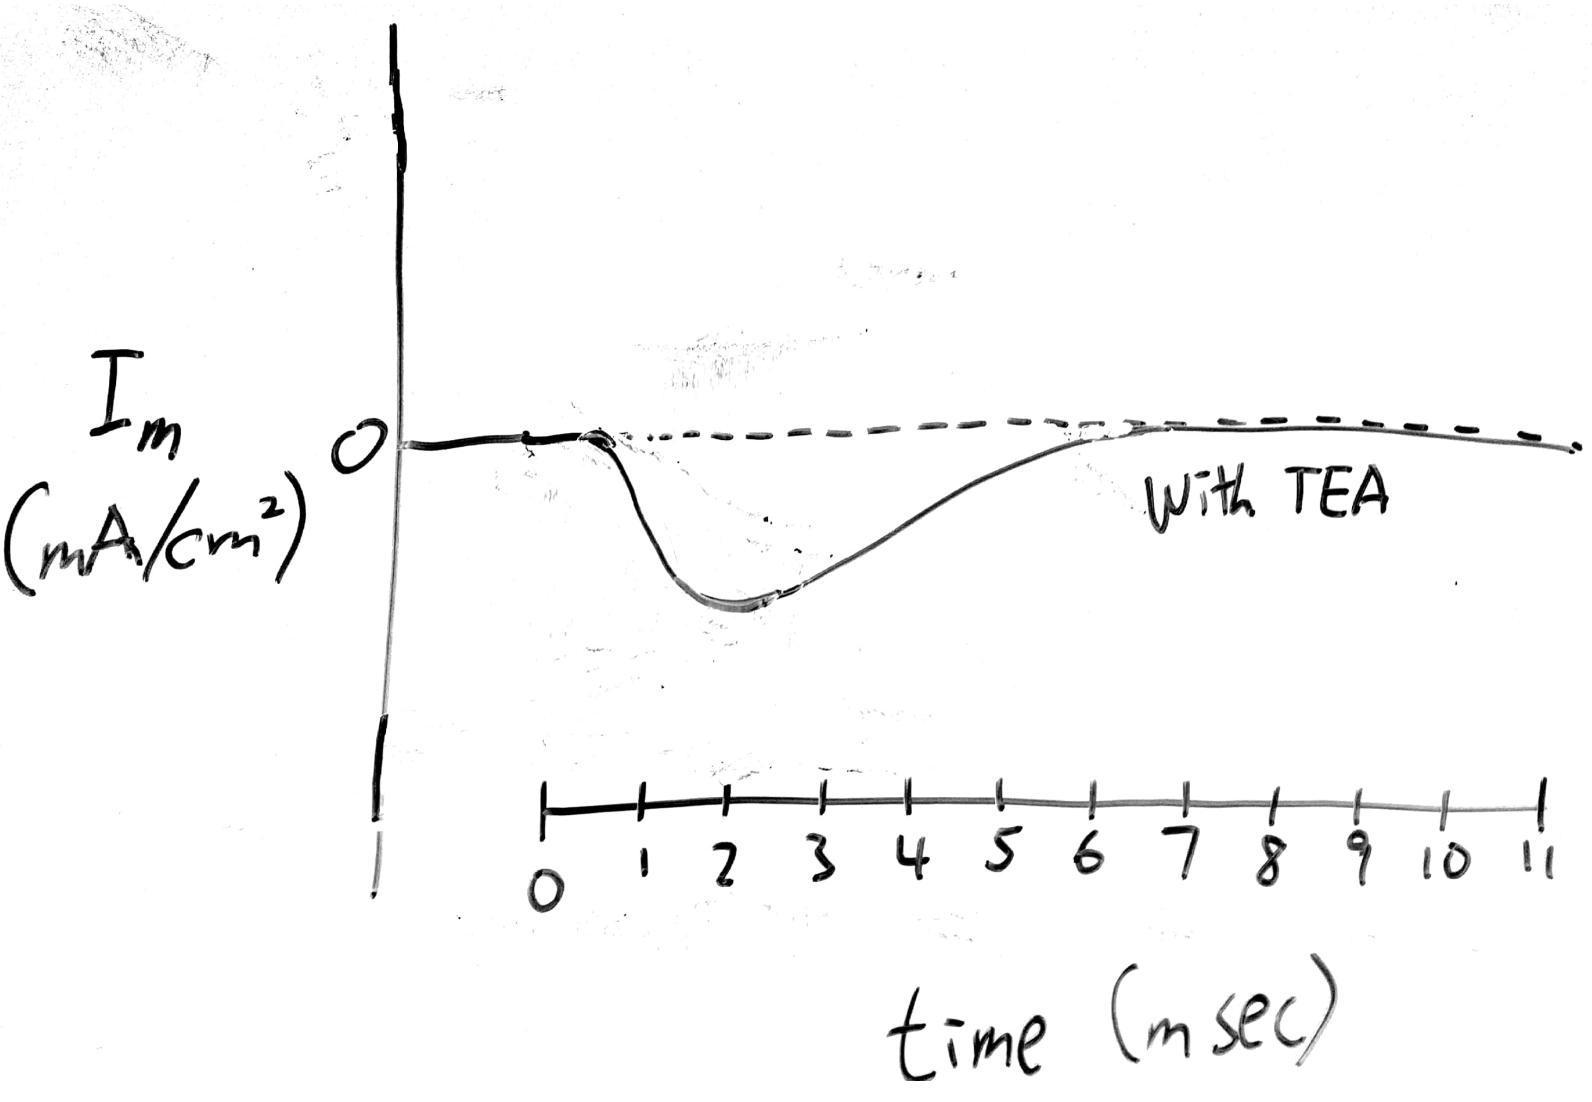
\includegraphics[width=0.5\textwidth]{/Users/jonathansun5/Documents/Fall 2017/MCB 166/Homeworks/HW 4/Screen Shot 2017-10-30 at 9.19.05 PM.png}
\end{center}



\item
$[\ch{Na+}]_{\text{out}}$ is adjusted so that $[\ch{Na+}]_{\text{out}} = [\ch{Na+}]_{\text{in}}$.
\vspace*{1\baselineskip}
\\
Because $[\ch{Na+}]_{\text{out}} = [\ch{Na+}]_{\text{in}}$, this is the same as if the \ch{Na+} channel was not in use and so the current will not go below 0.
\begin{center}
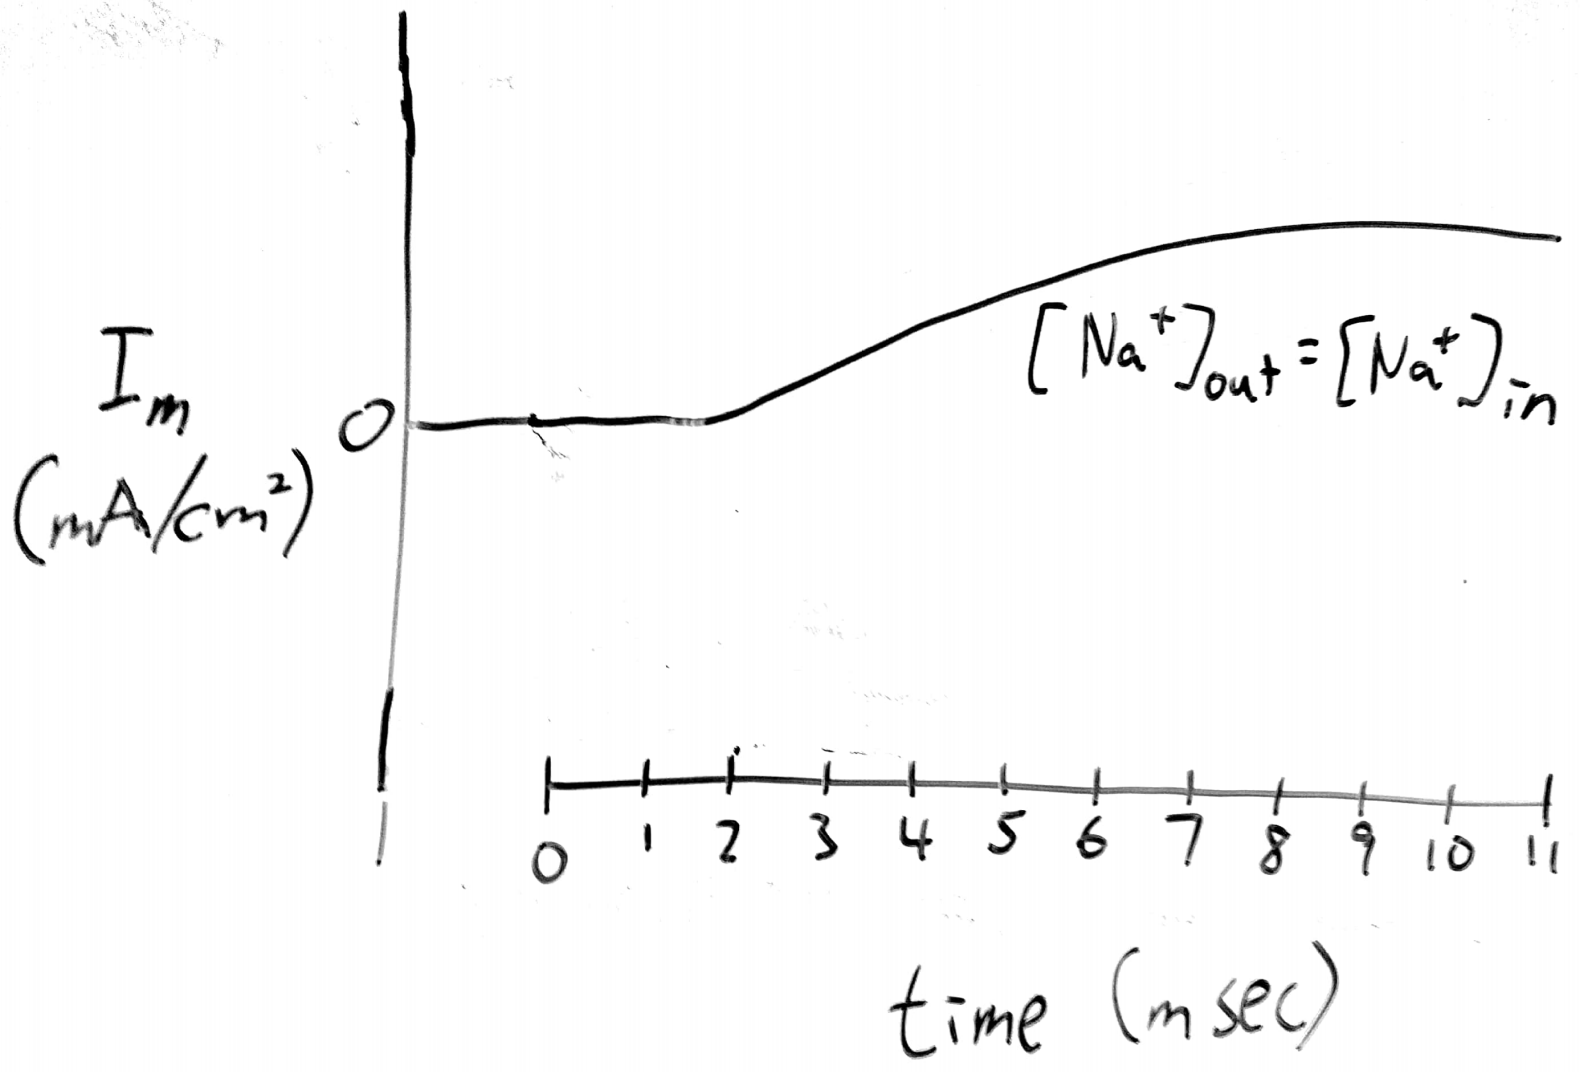
\includegraphics[width=0.5\textwidth]{/Users/jonathansun5/Documents/Fall 2017/MCB 166/Homeworks/HW 4/Screen Shot 2017-10-30 at 9.19.31 PM.png}
\end{center}



\item
$[\ch{K+}]_{\text{out}}$ is adjusted so that $[\ch{K+}]_{\text{out}} = [\ch{K+}]_{\text{in}}$.
\vspace*{1\baselineskip}
\\
Because $[\ch{K+}]_{\text{out}} = [\ch{K+}]_{\text{in}}$, this is the same as if the \ch{K+} channel was not in use and so the current will not go above 0.
\begin{center}
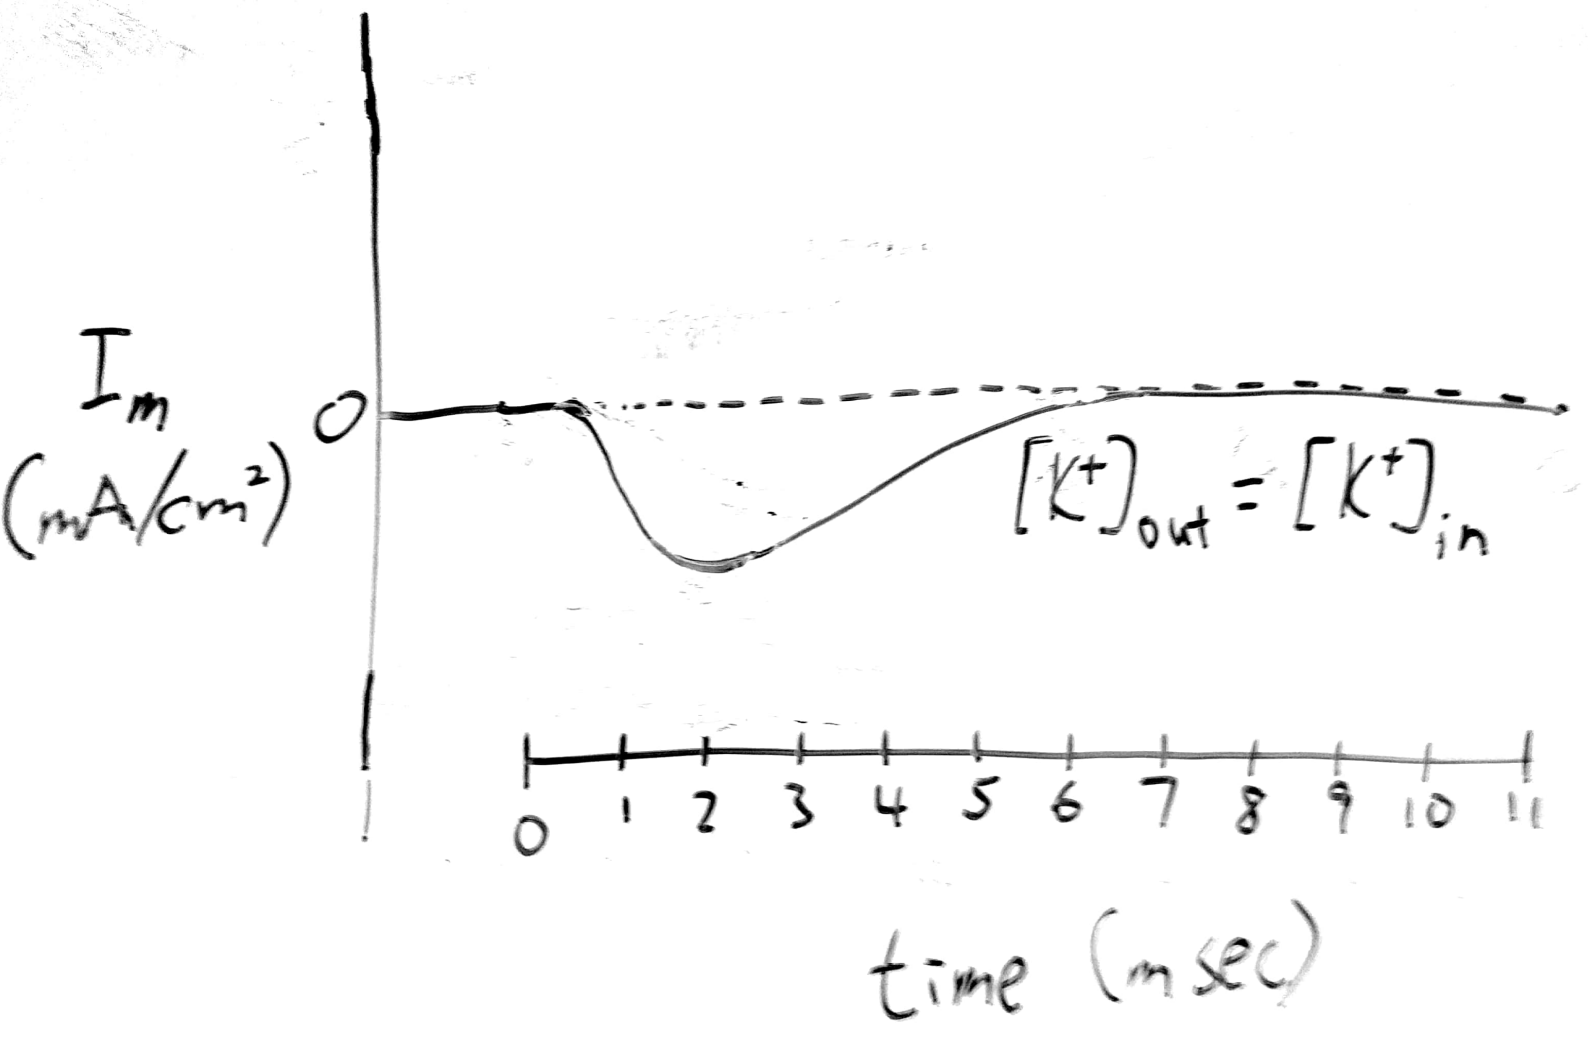
\includegraphics[width=0.5\textwidth]{/Users/jonathansun5/Documents/Fall 2017/MCB 166/Homeworks/HW 4/Screen Shot 2017-10-30 at 9.19.43 PM.png}
\end{center}



\item
Ouabain, a specific inhibitor of the \ch{Na+}-\ch{K+} pump, is added to the bath five minutes before the experiment.
\vspace*{1\baselineskip}
\\
Because Ouabain inhibits both \ch{Na+} and \ch{K+}, the current will neither be positive nor negative and so will stay as 0.
\begin{center}
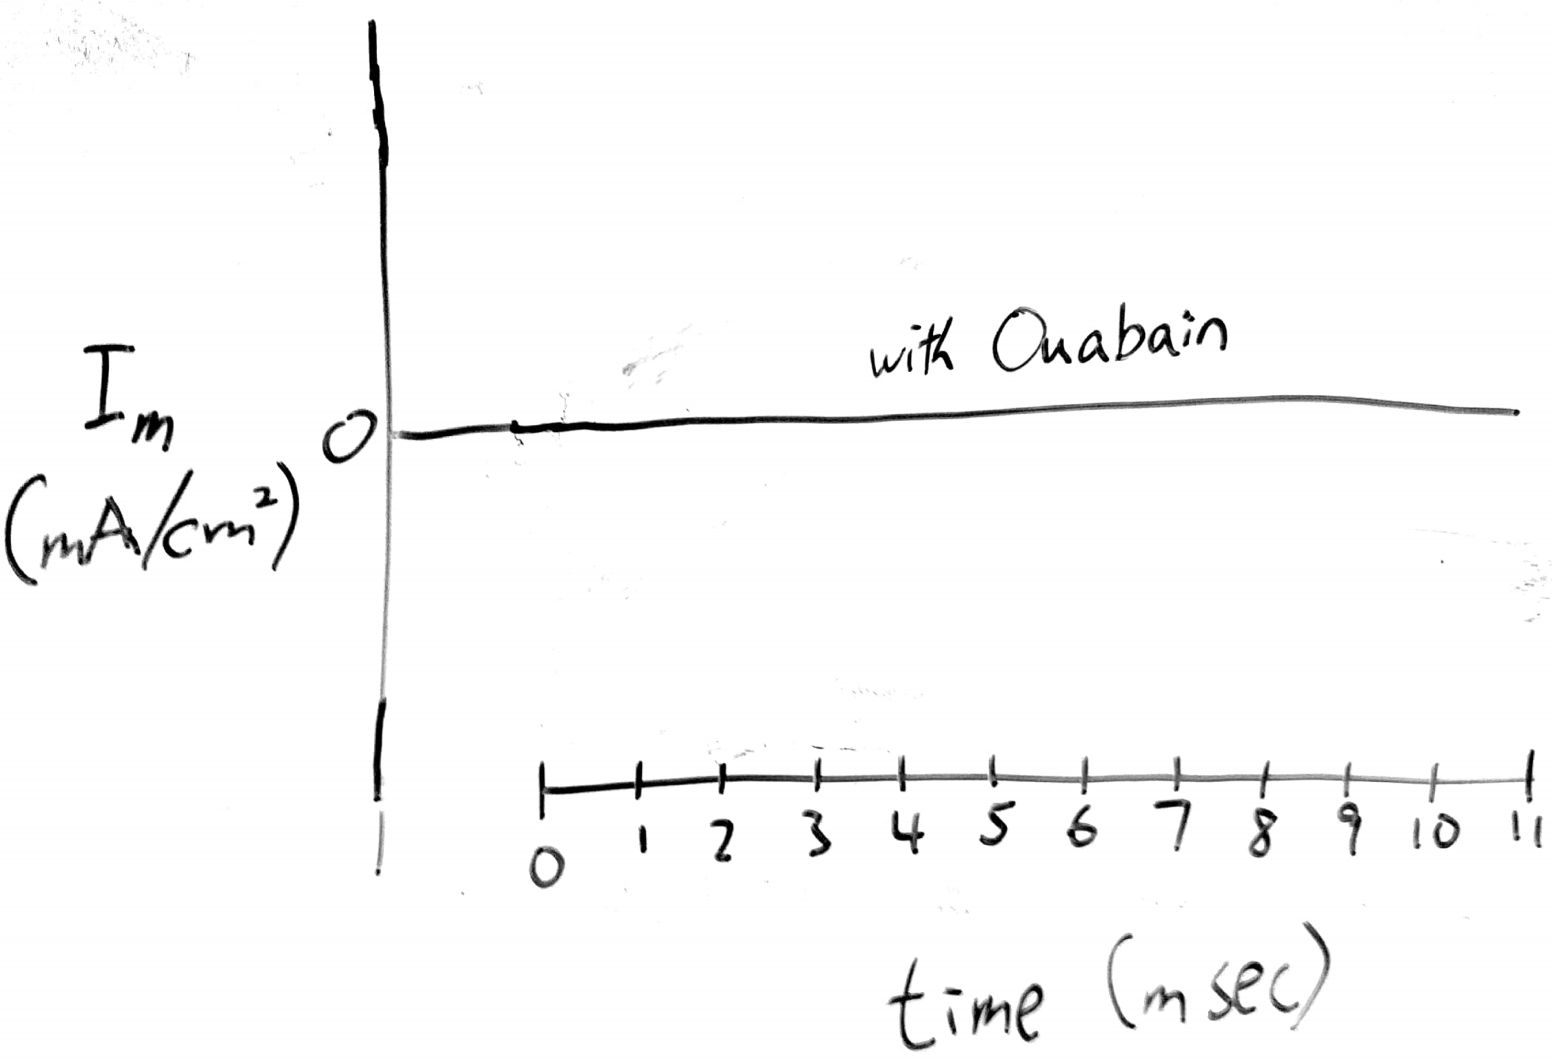
\includegraphics[width=0.5\textwidth]{/Users/jonathansun5/Documents/Fall 2017/MCB 166/Homeworks/HW 4/Screen Shot 2017-10-30 at 9.20.00 PM.png}
\end{center}
\end{enumerate}
\end{enumerate}
\end{document}
